\chapter{同伦和基本群}
“本章和以后各章所讲的都属于代数拓扑学的范畴.代数拓扑学的基本思想是对拓扑空间建立以代数概念(如群、交换群、环等)为形式的拓扑不变量,从而把代数方法引进拓扑学的研究中来.我们已说过,要判定空间不同胚,需要用拓扑性质(不变量).第二章中,我们已看到分离性、可数性、紧致性和连通性这些拓扑性质在这方面的应用.然而用这些概念能解决的问题毕竟太少了,本书至此已积累了不少尚未解决的重要问题,如\(E^N\)与\(E^m\)当n≠m时)是不是不同胚?与\(E^2\)的不同胚问题,\(S^2\)与\(T^2\)以及\(S^2\)与\(D^2\)等等不同胚的判定.在这许多问题上,代数拓扑学将表现出它的威力.同伦论和同调论是代数拓扑学的两大支柱.本书中只能涉及到“它们的一些初步知识.同伦是同伦论的最基础的概念之一;基本群是1维同伦群,它是代数拓扑学中最简单,用途最广的部分.闭曲面分类定理尚未完成的那一半证明涉及到判定两个空间不同胚的问题.例如怎么证明直观上看,\(T^2\)有洞,可以用线拴住,球面拴不住.但这里并不是指拴它们的线圈能否移走(在4维空间中,栓环面的线圈也能移走),正确的解释为:球面上弹性极好的闭合线圈可以在球面上滑缩为一点,而在环面上有些闭曲线(如经圆或纬圆)不能在环面上滑缩为一点.类似的差别也出现在平环与圆盘的比较中.显然圆盘上的闭曲线可容易地在圆盘上收缩为一点,而平环上环绕着它的洞的闭曲线被洞阻挡而“缩不成一点(图\ref{fig:enter-label_18}).基本群就是在闭曲线的可收缩性这种直观背景的基础上发展起来的一种结构.拓扑学中用道路概念替代曲线.道路本身是一种连续映射.为了理解道路的收缩和变形的意义,先一般地介绍连续映射的变形,也就是同伦概念.”
\begin{figure}[H]
    \centering
    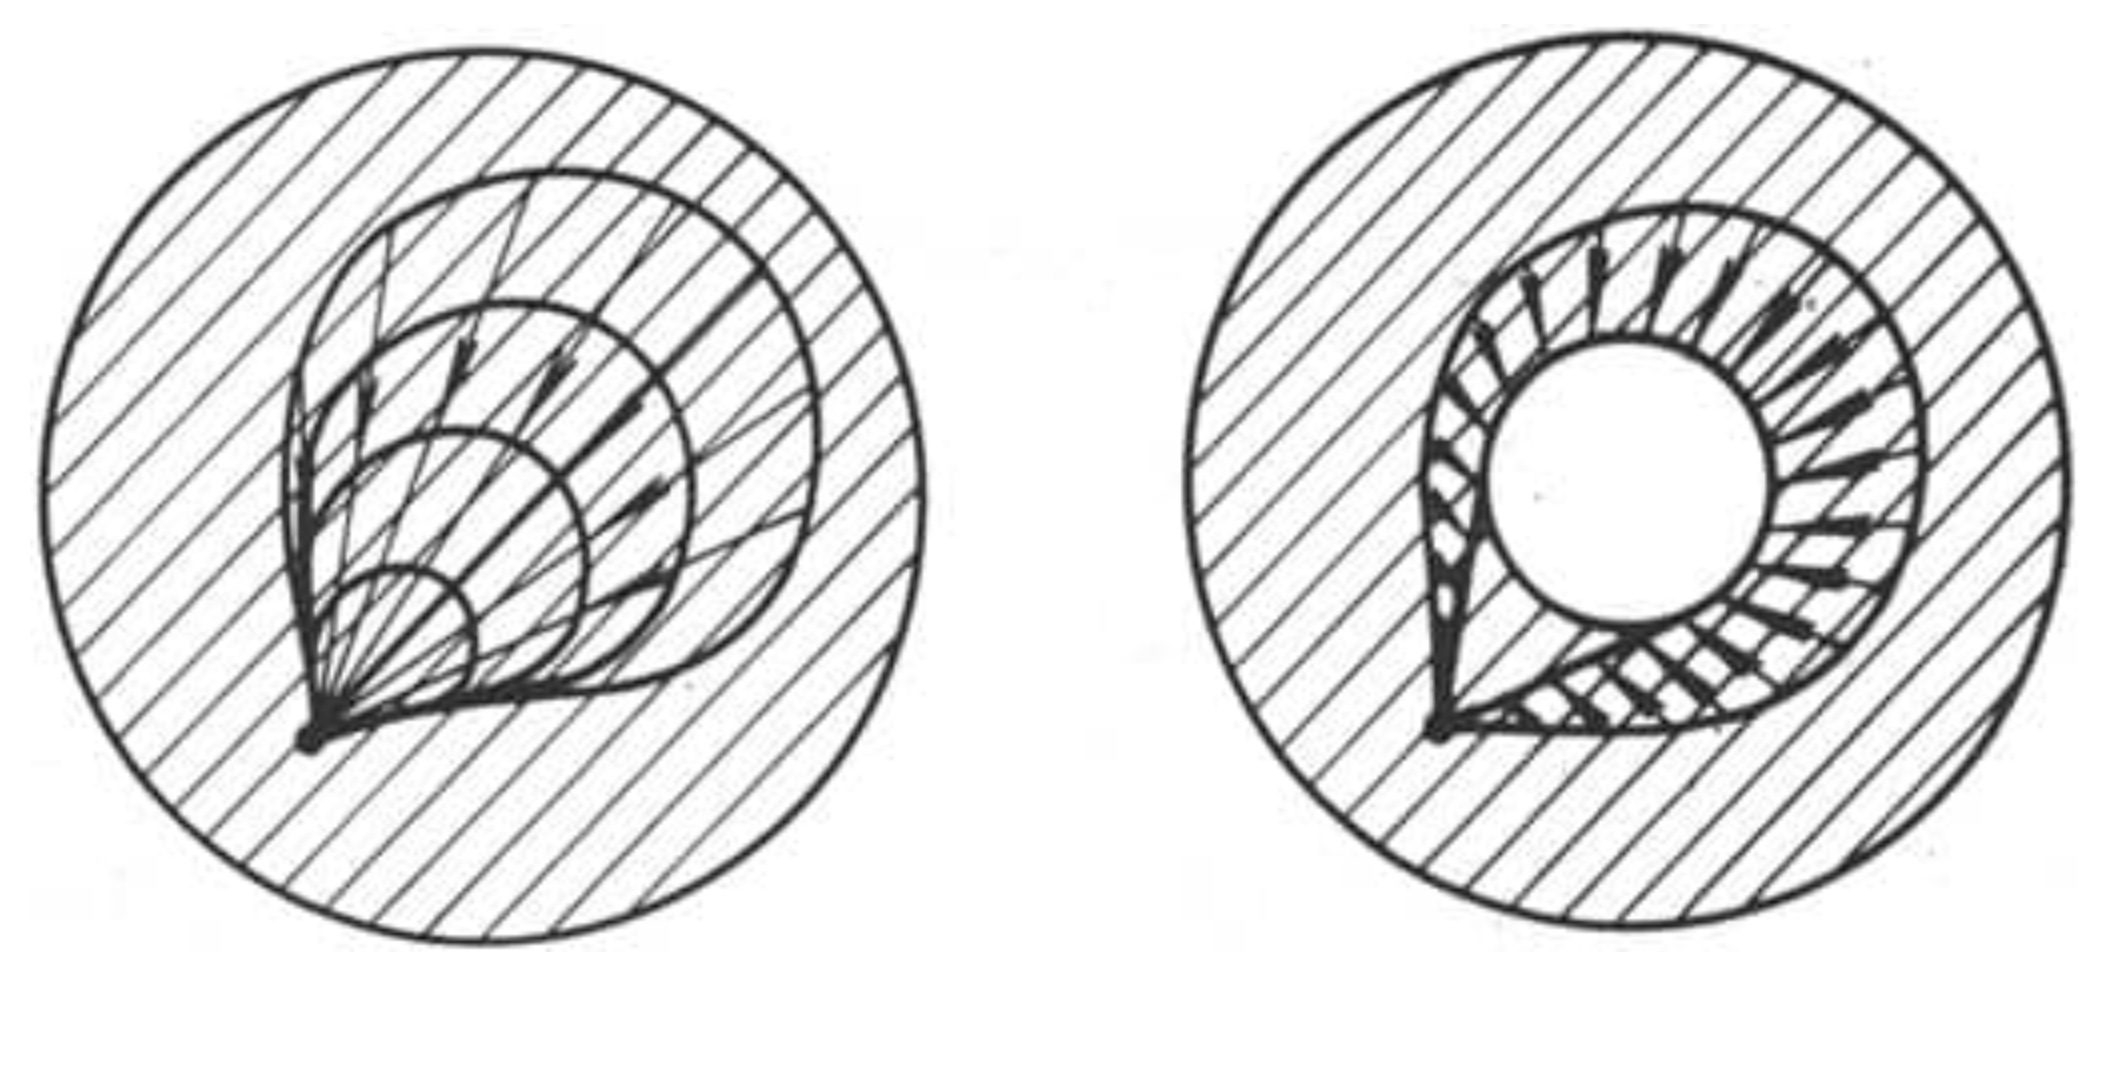
\includegraphics[width=0.5\linewidth]{image_18.png}
    \caption{}
    \label{fig:enter-label_18}
\end{figure}
\section{映射的同伦}
首先回顾一下同伦:
同伦就是映射之间的连续变形.设X与Y都是拓扑空间,记\(C(X,Y)\)是X到Y的所有连续映射的集合,设\(f,g \in C(X,Y)\),所谓f与g同伦,就是f可以“连续地”变化为g.因此有定义:
\begin{definition}
    设\(f ,g \in C(X,Y)\),如果有连续映射\(H: X \times I \rightarrow Y \),使得\(\forall x \in X , H(x,0) = f(x) , H(x.1) =g(x)\)则称f与g同伦.记作\(f \simeq g : X \rightarrow Y\),或者简记为\(f \simeq g\).称H是连接f和g的一个同伦,记作\(H: f \simeq g \) (或者 \(f \overset{H}{\simeq}g \) 
\end{definition}
对于每个\(t \in I \),同伦H决定\(h_t \in C (X,Y) \)为 \(h_t(x) = h(x,t)\),于是得到单参数连续映射族\(\left\{h_t | t \in I \right\}\),称\(h_t\)为H的t-切片.根据定义\(h_0 =f \quad h_1 = g\)(如图\ref{fig:enter-label_19})
\begin{figure}[H]
    \centering
    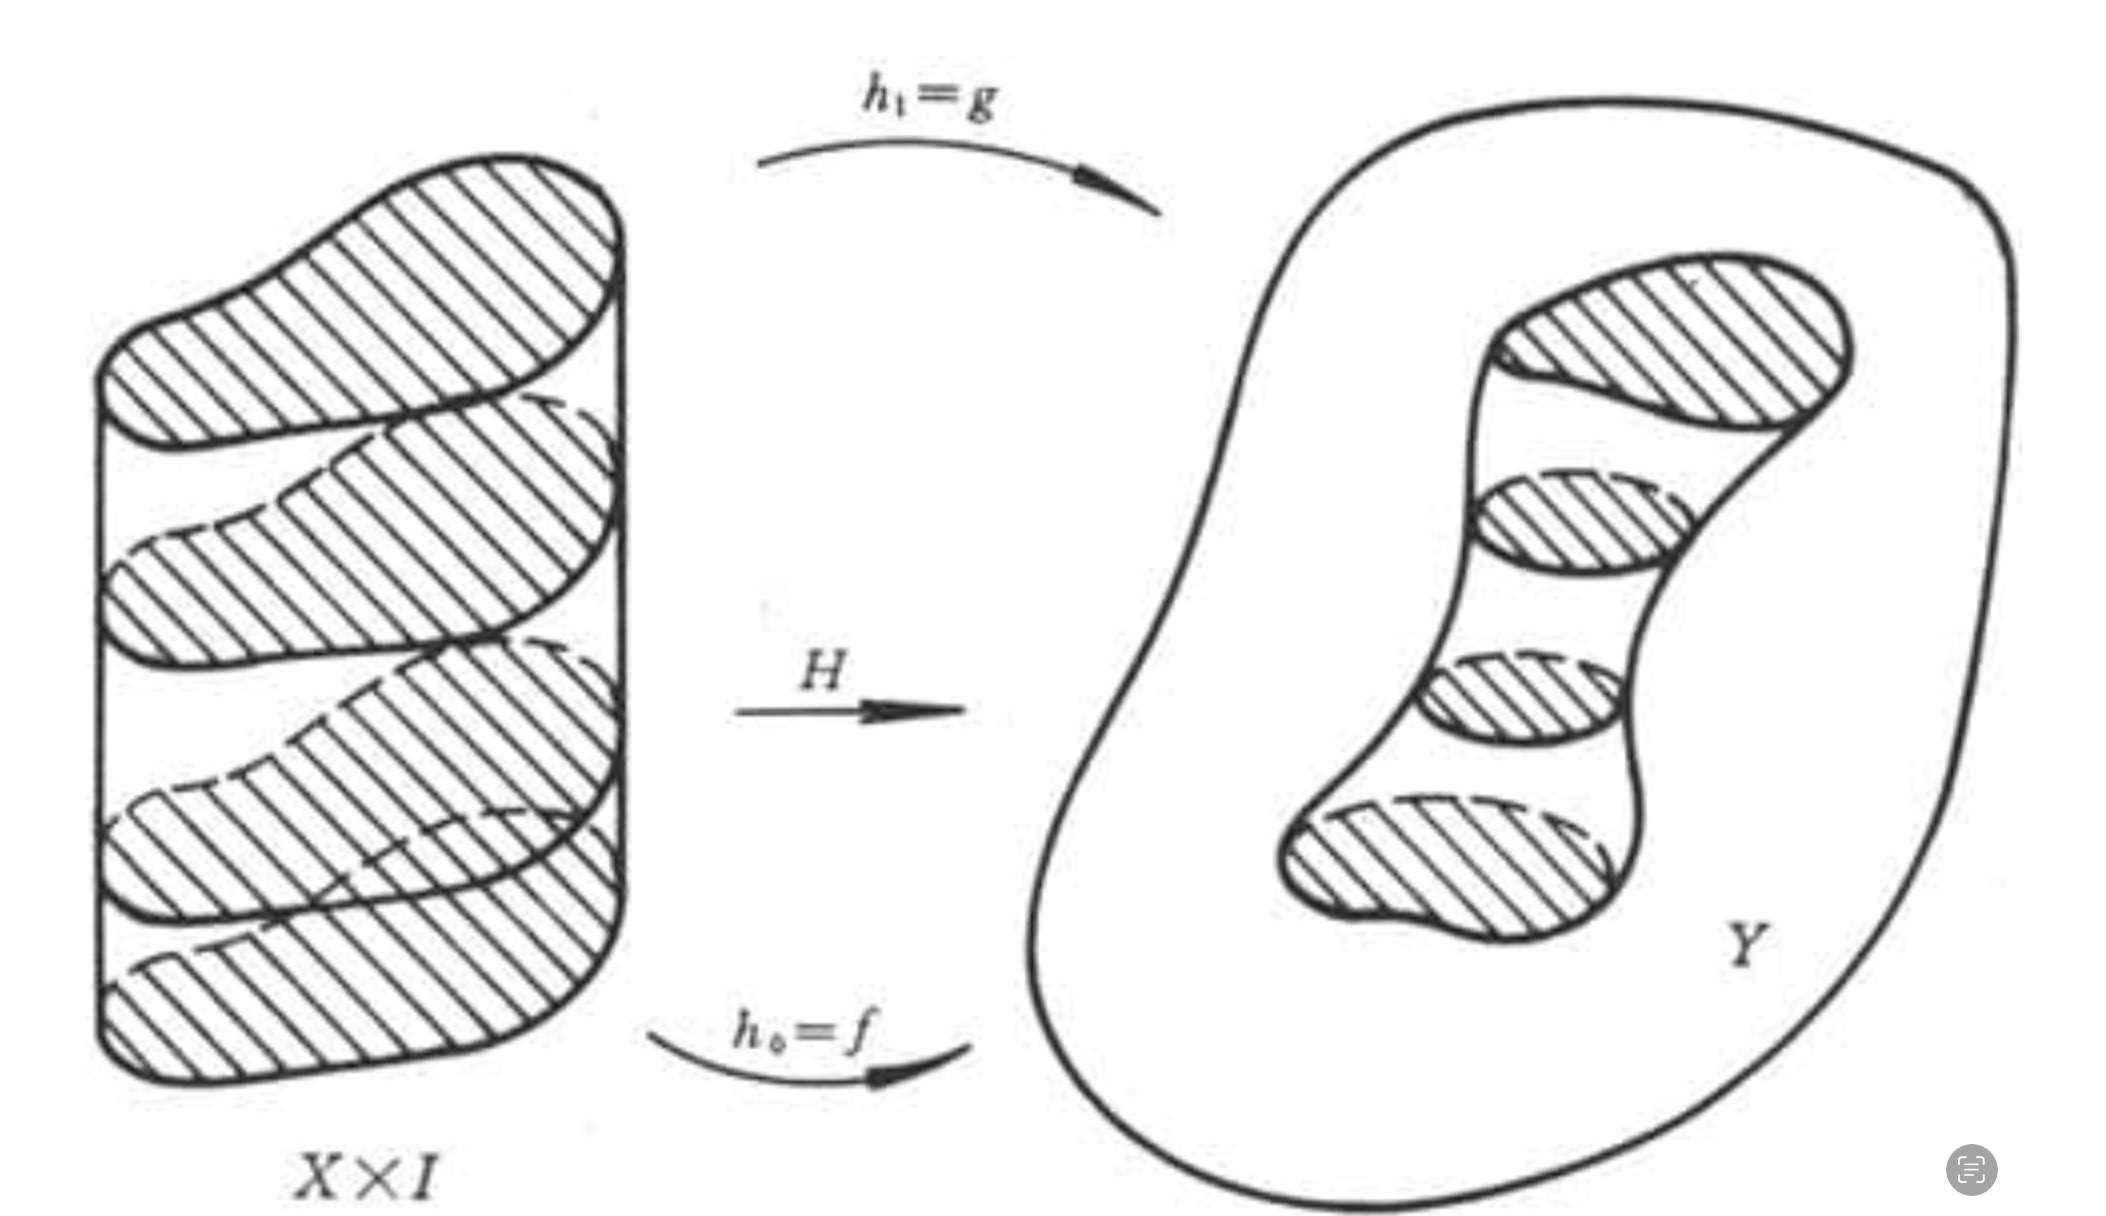
\includegraphics[width=0.5\linewidth]{image_19.png}
    \caption{}
    \label{fig:enter-label_19}
\end{figure}
下面给出几个同伦的例子
\begin{example}
    设\(f,g \in C(X,E^n)\),规定\(H: X \times I \rightarrow E^n\)为
    \[H(x,t) = (1-t) f(x) +tg(x)\]
    易知H是f到g的同伦
\end{example}
\begin{note}
    上述是我们考虑函数同伦的基础,应好好理解
\end{note}
\begin{example}
    若\(f,g \in C(X ,S^n)\),使得\(\forall x \in X  \quad f(x) \neq -g(x) \),则可规定f到g的同伦H为
    \begin{align}
        H(x,t) = \frac{(1-t)f(x) + tg(x)}{\parallel (1-t)f(x) + tg(x) \parallel }
    \end{align}
    
\end{example}
如果f同伦于一个常值映射,则称f是零伦的.
\begin{definition}
    设\(A \subset X \quad f,g \in C(X,Y)\),如果存在f到g的同伦H,使得当\(a \in A \)时,\(H(a,t)=f(a)=g(a) , \quad \forall t \in I \),则称f和g相对于A同伦,记作\(f \simeq g \quad \text{relA} \),称H是f到g的相对于A的同伦,记作\(H: f \simeq g \quad \text{relA}\)(或\(f \overset{H}{\simeq} \quad \text{relA}\)
\end{definition}
\begin{corollary}
    取定\(A \subset X\),则\(C(X,Y)\)中相对于A的同伦也是等价关系.
\end{corollary}
\begin{corollary}
    设\(f_0 \simeq f_1: X \rightarrow Y \quad \text{relA}\),\(g_0 \simeq g_1 : Y \rightarrow Z \text{relB}\),并且\(f_0(A) \subset B\),则\(g_0 *f_0 \simeq g_1 *f_1 \quad \text{relA}\)
\end{corollary}
\begin{definition}
    设a,b是X上的两条道路,如果 \(a \simeq b \text{rel} \left\{0,1\right\}\),则称a与b定端同伦,记作 \(a \underset{.}{\simeq} b  \)
\end{definition}
显然\(a \underset{.}{\simeq} b\)的一个必要条件是a与b有相同的起终点,a到的一个定端同伦是从矩阵\(I \times I \)到X的一个连续映射,它把左右侧边分别映为a(0)和a(1) ,在下底和上底上的限制分别是道路a与b(如图\ref{fig:enter-label_20})
\begin{figure}[H]
    \centering
    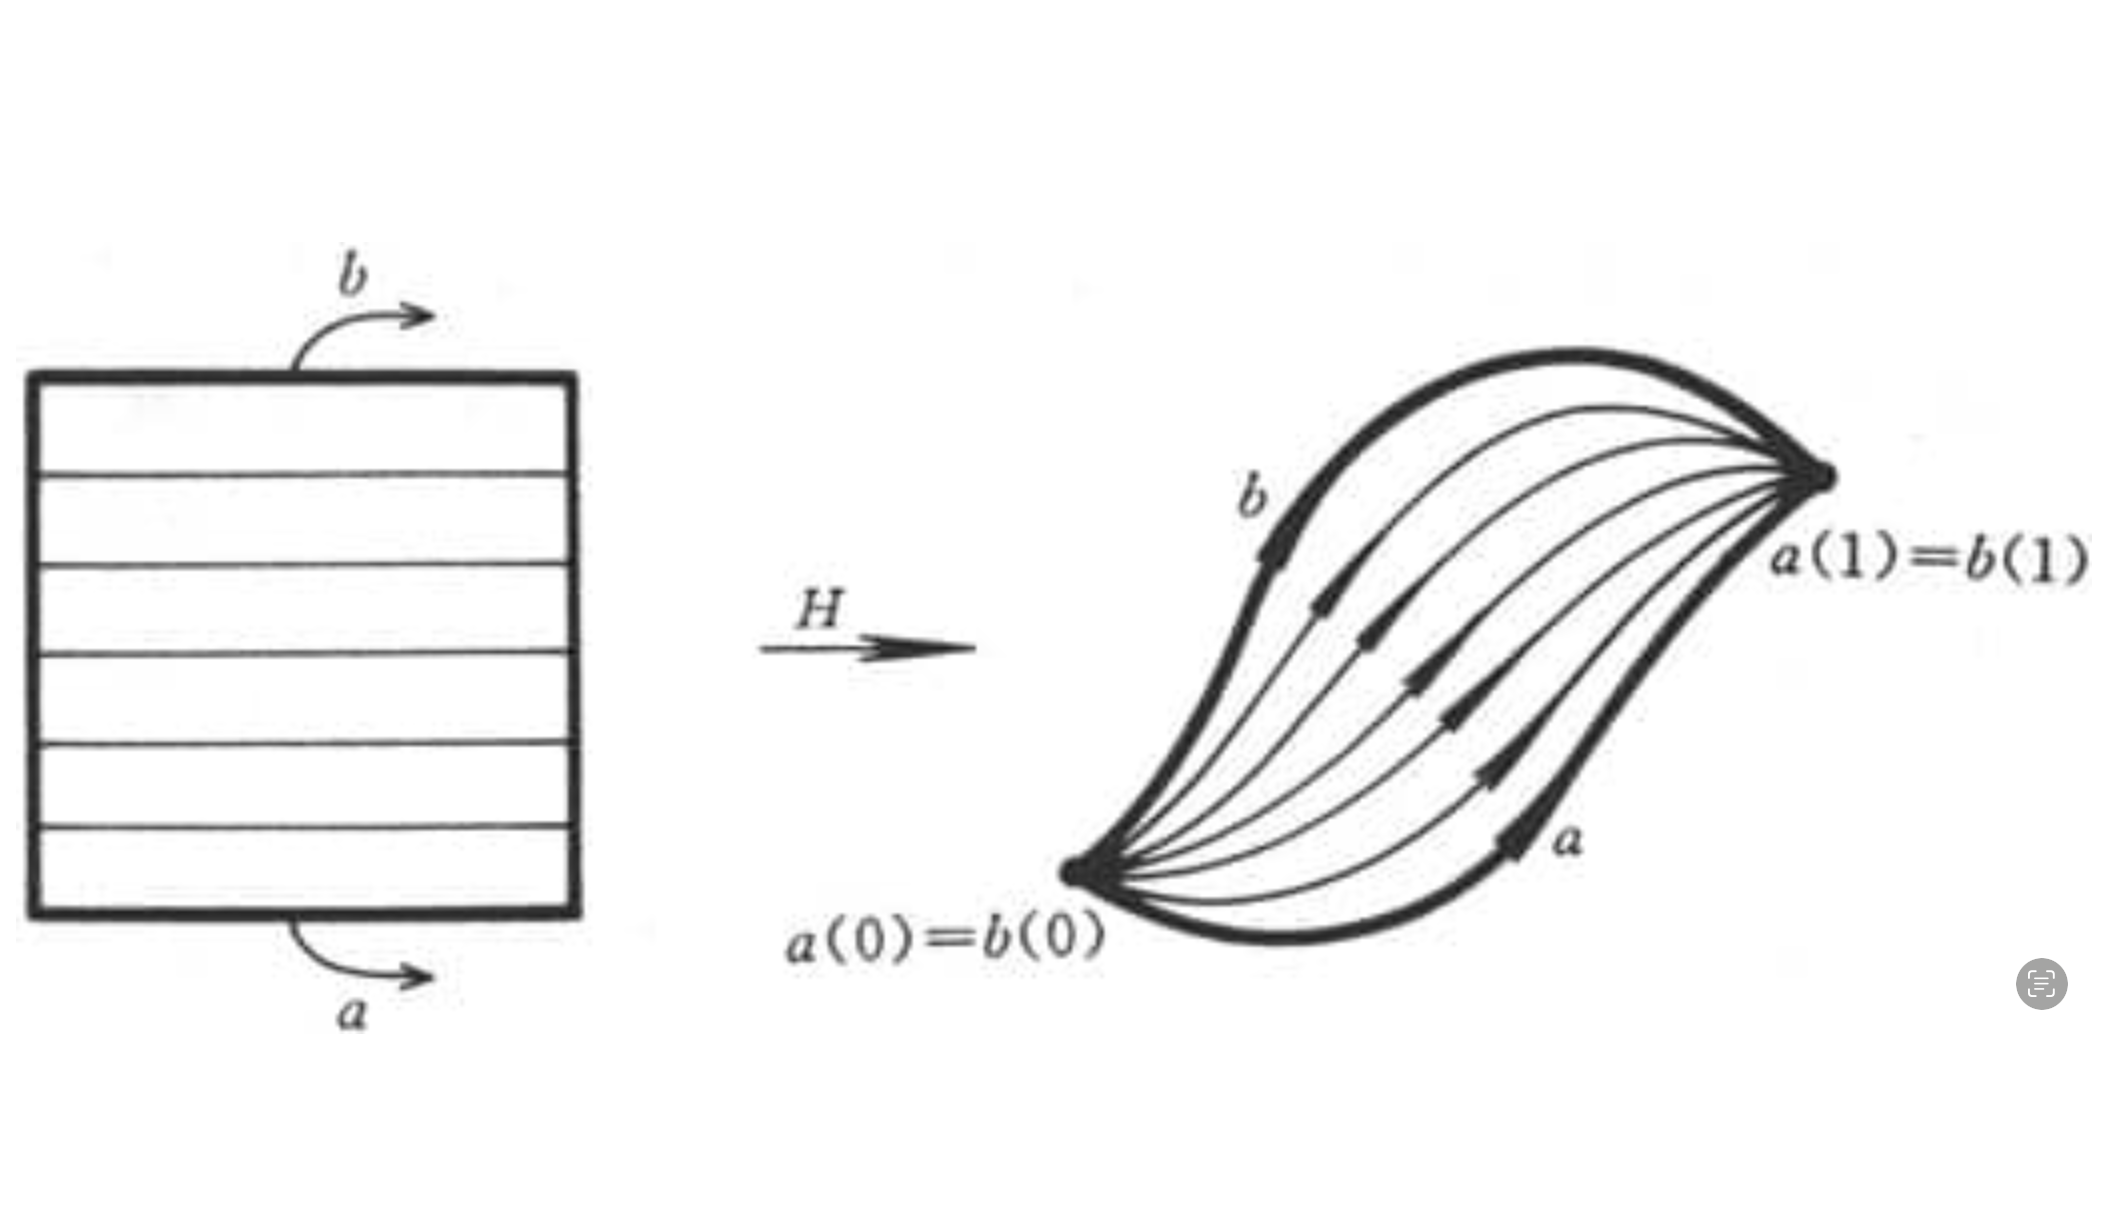
\includegraphics[width=0.3\linewidth]{image_20.png}
    \caption{}
    \label{fig:enter-label_20}
\end{figure}
X的所有道路在\(\underset{.}{\simeq}\)关系下分成的等价类称为X的道路类,X的所有道路类的集合记作[X],一条道路a所属的道路类记作<a>,称a的起终点,起终点重合的道路类称为闭路类,称起(终)点为它的基点.
\begin{theorem}
    连续映射\(f: X \rightarrow Y \)零伦\(\Leftrightarrow\) f可以扩张到\(C_X\)上
\end{theorem}
\begin{theorem}
    设\(f:X \rightarrow Y\)连续,X中道路\(a \underset{.}{\simeq} b\),则\(f*a \underset{.}{\simeq} f *b\)
\end{theorem}
\section{基本群的定义}
“基本群是在道路及其运算(逆和乘积)的基础上建立的.但道路不能直接当作元素来建立群.有两个问题:一是道路的乘法没有结合律;二是并非任何两条道路都可相乘.我们用道路类替代道路,解决了第一个问题;用取定基点的办法解决第二个问题.”
\subsection*{道路类的逆和乘积}
\begin{corollary}
    \begin{enumerate}
        \item 如果 \(a \underset{.}{\simeq}b \),则 \(\overline{a} \underset{.}{\simeq} \overline{b}\) \\
        \item 如果 \(a \underset{.}{\simeq} , c\underset{.}{\simeq}d\),并且ac有意义,则 \[ac \underset{.}{\simeq} bd\] \\
    \end{enumerate}
\end{corollary}
\begin{definition}
    \begin{enumerate}
        \item 规定道路类\(\alpha\)的逆\(\alpha^{-1} = < \overline{\alpha}> \),其中 \(\alpha \in a \) \\
        \item 若道路类\(\alpha\)的终点与\(\beta\)的起点重合,规定\(\alpha\)与\(\beta\)的乘积\(\alpha\beta = <ab> \),其中 \(a \in \alpha ,b \in \beta\)
    \end{enumerate}
\end{definition}
\(\alpha^{-1}\)的起点和终点分别是\(\alpha\)的终点和起点 ; \(\alpha \beta\)的起点和终点分别是\(\alpha\)的起点和\(\beta\)的终点
由道路逆和乘积的性质 : \(\overline{\overline{a}}= a  ; \overline{ab}=\overline{b}\overline{a}\).
\subsection*{道路类运算的性质}
\begin{corollary}
    设\(f: X \rightarrow Y\)是连续映射,a,b是X上两条道路.
    \begin{enumerate}
        \item 如果\(a \underset{.}{\simeq} b \),则 \(f * a \underset{.}{\simeq} f* b \) \\
        \item 如果a与b可乘,则\(f*a\)与\(f*b\)也可乘,并且 \[(f*a)(f*b) = f*(ab)\] ; \\
        \item \(\overline{f*a} = f * \overline{a} \) 
    \end{enumerate}
\end{corollary}
\begin{corollary}
    道路类乘法有结合律
\end{corollary}
\begin{corollary}
    设道路类\(\alpha\)的起终点分别是\(x_0\)和\(x_1\),记\(e_{x_0}, e_{x_1}\)分别是=\(x_0 , x_1\)处的点道路,则
    \begin{enumerate}
        \item \(\alpha\alpha^{-1} = <e_{x_0}> , \quad \alpha^{-1}\alpha = <e_{x_1}> \) \\
        \item \(<e_{x_0}> \alpha = \alpha = \alpha <e_{x_1}>\)
    \end{enumerate}
\end{corollary}
上述命题说明点道路所在道路类具有单位性 .
\subsection*{空间的基本群和连续映射诱导的基本群的同态}
设X是一个拓扑空间,取定\(x_0 \in X \),把X的以\(x_0\)为基点的所有闭路类的集合机组\(\pi_1(X ,x_0)\).于是\(\pi_1(X,x_0)\)中任何两个元素都是可乘的,乘积仍在\(\pi_1(X,x_0)\) . 
\begin{definition}
    称z\(\pi_1(X,x_0)\)在道路类乘法运算下构成的群为X的以\(x_0\)为基点的基本群
\end{definition}
\begin{example}
    设X是\(E^n\)的凸集,\(x_0 \in X \)是任一点,因为\(x_0\)处任意的两条闭路都定端同伦,所以\(\pi_1(X,x_0)\)只有一个元素安,它是一个平凡群
\end{example}
\begin{definition}
    如果\(f: X \rightarrow Y \)连续,\(x_0 \in X  \quad y_0 =f(x_0)\),称同态\(f_{\pi} :  \pi_1(X,x_0) \rightarrow \pi_1(Y,y_0) \) 为f诱导出的基本群同态 .
\end{definition}
\begin{note}
    注意这里基点\(x_0\)是可以任意取的,因此f诱导出许多基本群同态(对于每一个点\(x \in X \)有一个同态),它们都记作\(f_{\pi}\) . 
\end{note}
\begin{corollary}
    设\(f: X \rightarrow Y  ; g: Y \rightarrow Z \)都是连续映射,\(x_0 \in X , y_0 = f(x_0) , z_0 = g(y_0)\) 则
    \[(g*f)_{\pi} = g_{\pi} * f_{\pi} : \pi_1(X,x_0) \rightarrow \pi_1 (Z,z_0)\]
\end{corollary}
\begin{theorem}
    若\(f: X \rightarrow Y\)是同胚映射,\(x_0 \in X , y_0 = f(x_0) \), 则\(f_{\pi} \pi_1 (X,x_0) \rightarrow \pi_1 (Y ,y_0)\)是同构. 
\end{theorem}
上述定理阐释:基本群是拓扑不变量
\subsection*{基本群与基点的关系}
基本群是由空间和基点共同决定的,那么同一空间在不同基点处的基本群有什么关系:给出下面定理: 
设\(x_0 ,x_1 \)是在X的同一道路分支中的两点,设\(\omega\)是从\(x_0\)到\(x_1\)的一个道路类.\(\forall \alpha \in \pi_1 (X,x_0), \omega^{-1}\alpha\omega \in \pi_1 (X ,x_1) \).于是,由\(\omega_{text{\#}}(\alpha) = \omega^{-1}\alpha\omega \)规定了\(\omega_{text{\#}} : \pi_1(X,x_0) \rightarrow \pi_1 (X.x_1)\)(图\ref{fig:enter-label_21})
\begin{figure}[H]
    \centering
    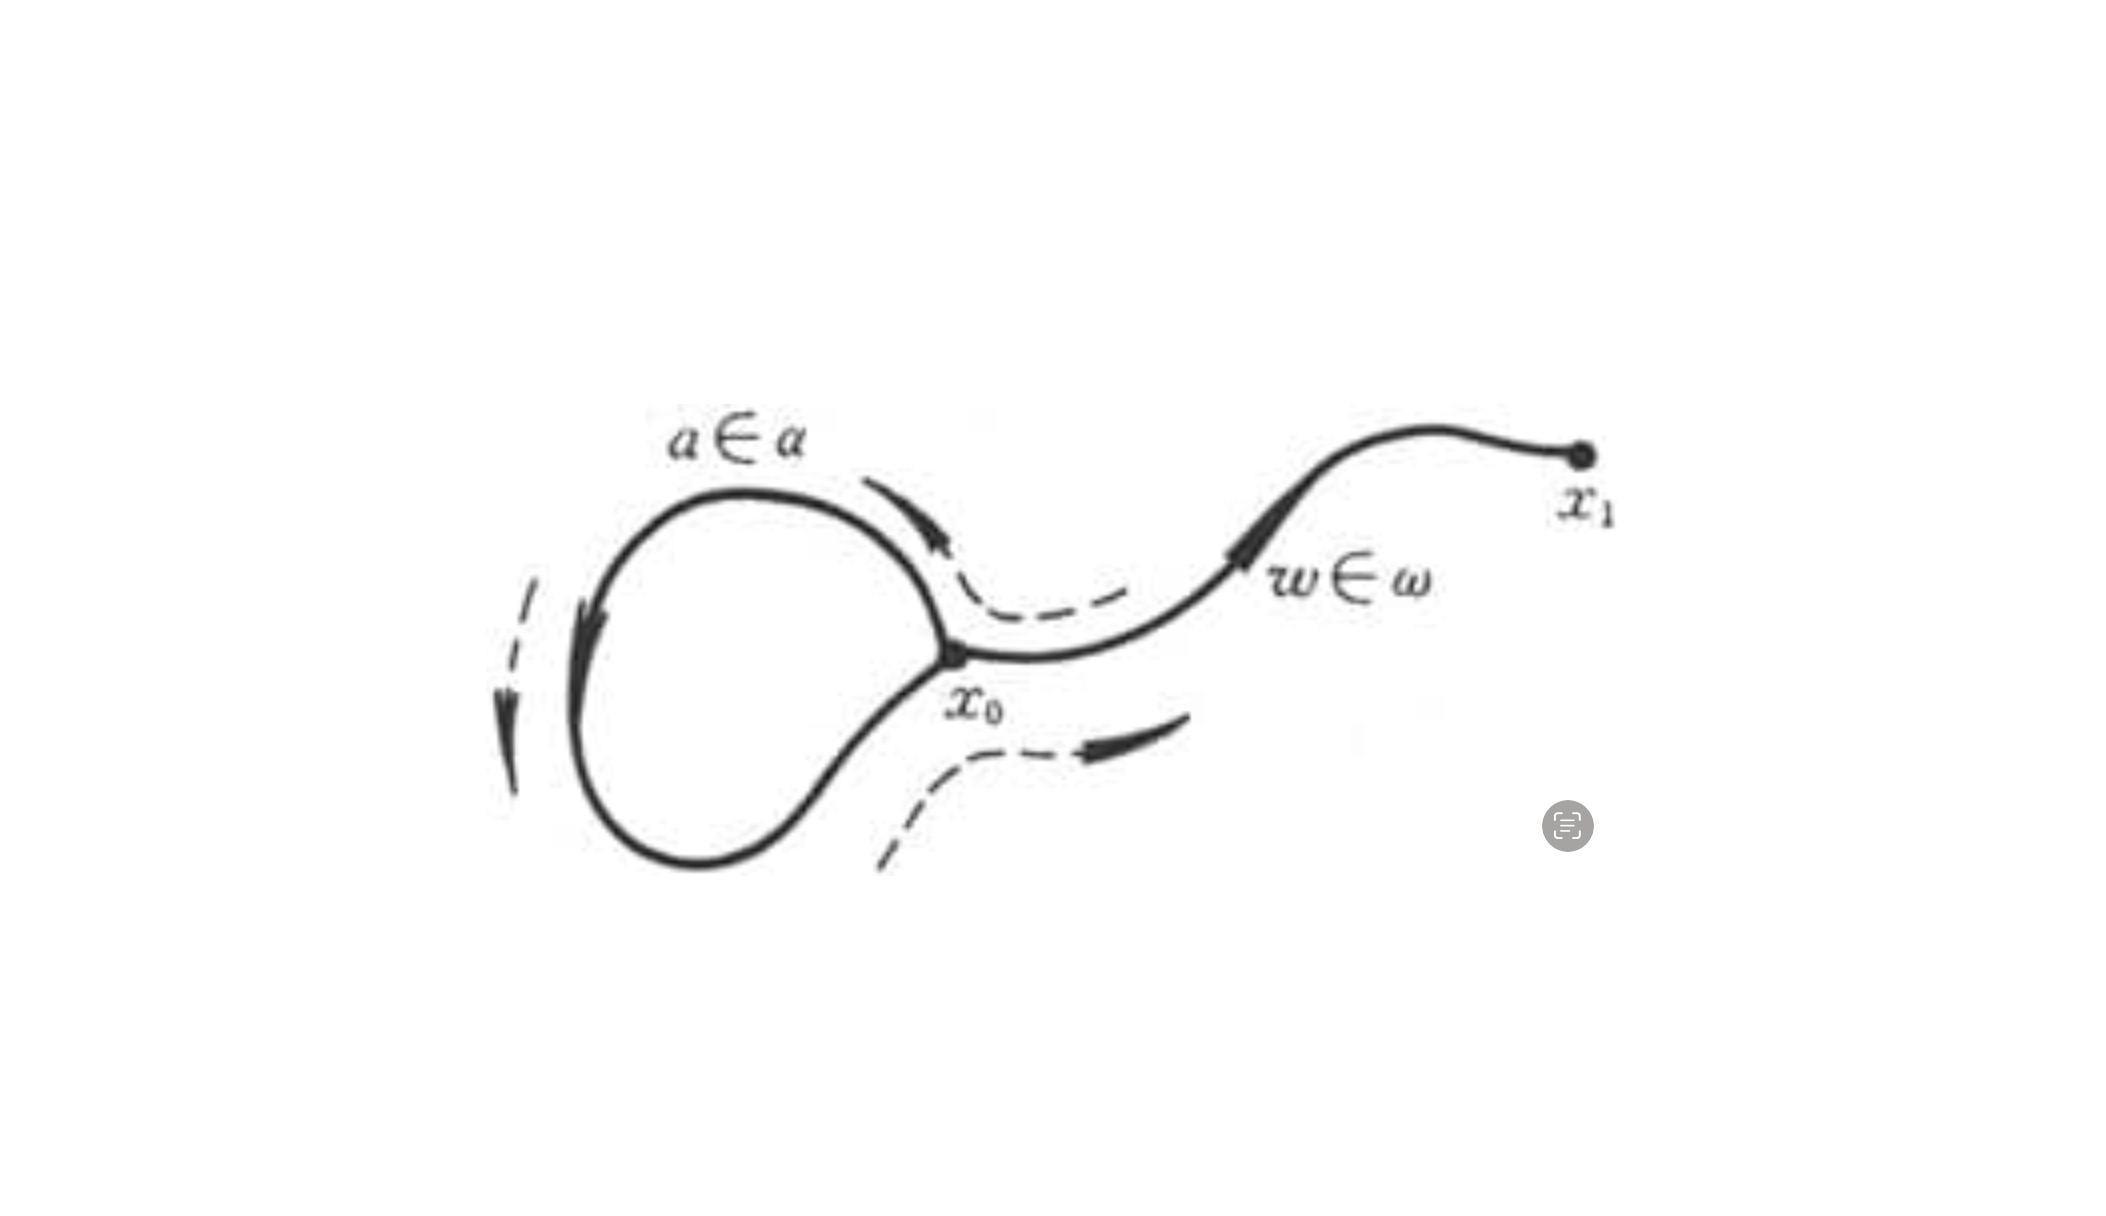
\includegraphics[width=0.5\linewidth]{image_21.png}
    \caption{}
    \label{fig:enter-label_21}
\end{figure}
\begin{theorem}
    若\(\omega\)是从\(x_0\)到\(x_1\)的道路类,则 
    \begin{enumerate}
        \item 如果\(\omega^{'}\)是从\(x_1\)到\(x_2\)的道路类,则
        \((\omega\omega_{\#} = w^{'}_{\#} * \omega_{\#} : \pi_1 (X,x_0) \rightarrow \pi_1 (X ,x_1)\) \\
        \item \(\omega_{\#} : \pi_1 (X,x_0) \rightarrow \pi_1 (X ,x_1)\)
    \end{enumerate}
\end{theorem}
\begin{definition}
    道路连通并有平凡基本群的拓扑空间称为单连通空间 . 
\end{definition}
\begin{corollary}
    设A是X的一个道路分支,\(x_0 \in A \), \(i : A \rightarrow X\)是包含映射, 则
    \[i_{\pi} : \pi_1 (X,x_0) \rightarrow \pi_1 (X ,x_1)\]
    是同构
\end{corollary}
\begin{theorem}
    设\(\omega_{\#} , \omega^{'}_{\#}\)是\(x_0\)到\(x_1\)的两个道路类.则: 
    \(\omega_{\#} =\omega^{'}_{\#} \Leftrightarrow \omega\omega^{'}\text{在}\pi_1(X,x_0) \text{的中心里}\)
\end{theorem}
\section{\(S^n\)的基本群}
“基本群的定义不是构造性的,不能用来计算基本群.事实上也不存在对任何空间都有效的一般计算方法.因此基本群的计算就成为我们所面临的问题.许多有效的方法都是利用基本群的性质以及一些技巧,把所作计算转化为求较简单空间的基本群.当然,这些较简单空间的基本群必须会算.本节所讲的\(S^n\)的基本群就经常作为求其他空间基本群的基础.”
\subsection*{\(S^1\)的基本群}
\(S^1\)的基本群主要依旧是作为基本来计算复杂的空间. \\
把\(S^1\)看作复平面上的单位圆,\(S^1 = \left\{z \in C | ||z|| =1 \right\}\).取\(z_0 = 1 \in S^1\)作基点.设a是基点为\(z_0\)的闭路,当t从0变到1时,\(a(t)\)从\(z_0\)出发在\(S^1\)上运动,并回到\(S^1\).规定连续映射\(p : E^{'} \rightarrow S^1\),为\(p(t) = e^{i2\pi t}\),它在计算中的作用十分强大.p在局部上是同胚的;记\(J_t = (t,t+1)\),则\(p|J_t \rightarrow S^1\)是嵌入映射.如图\ref{fig:enter-label_22}
\begin{figure}[H]
    \centering
    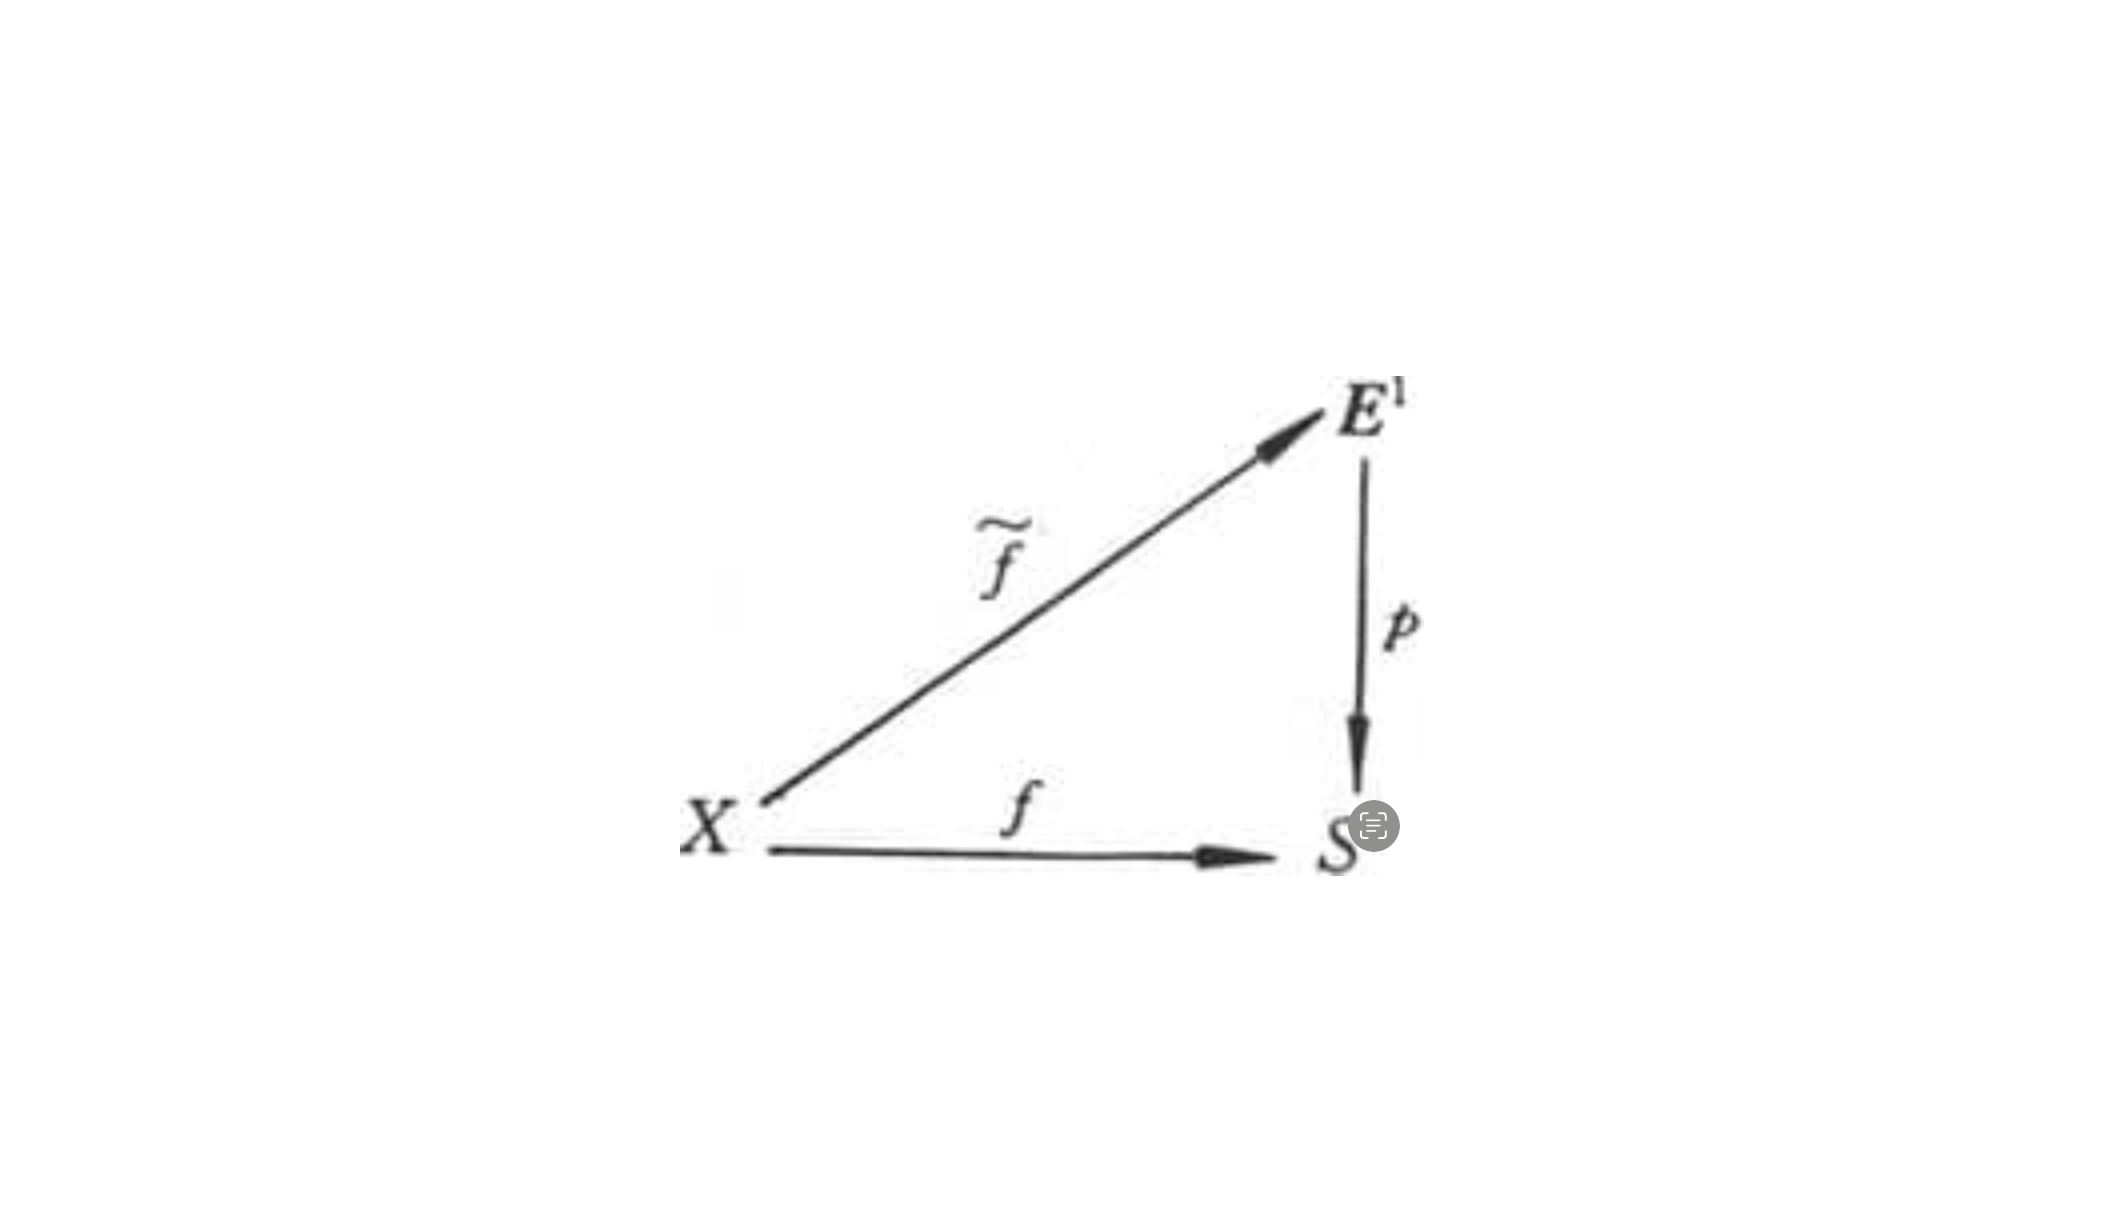
\includegraphics[width=0.5\linewidth]{image_22.png}
    \caption{映射流程图}
    \label{fig:enter-label_22}
\end{figure}
设X是拓扑空间,\(f: X \rightarrow S^1\)连续,X到\(E^1\)的连续映射\(\widetilde{f} : X \rightarrow  E^1\) 如果满足\(p * \widetilde{f} = f \),即左面的映射图表可以交换,则称\(\widetilde{f}\)是f的一个提升(图\ref{fig:enter-label_23}).
\begin{figure}[H]
    \centering
    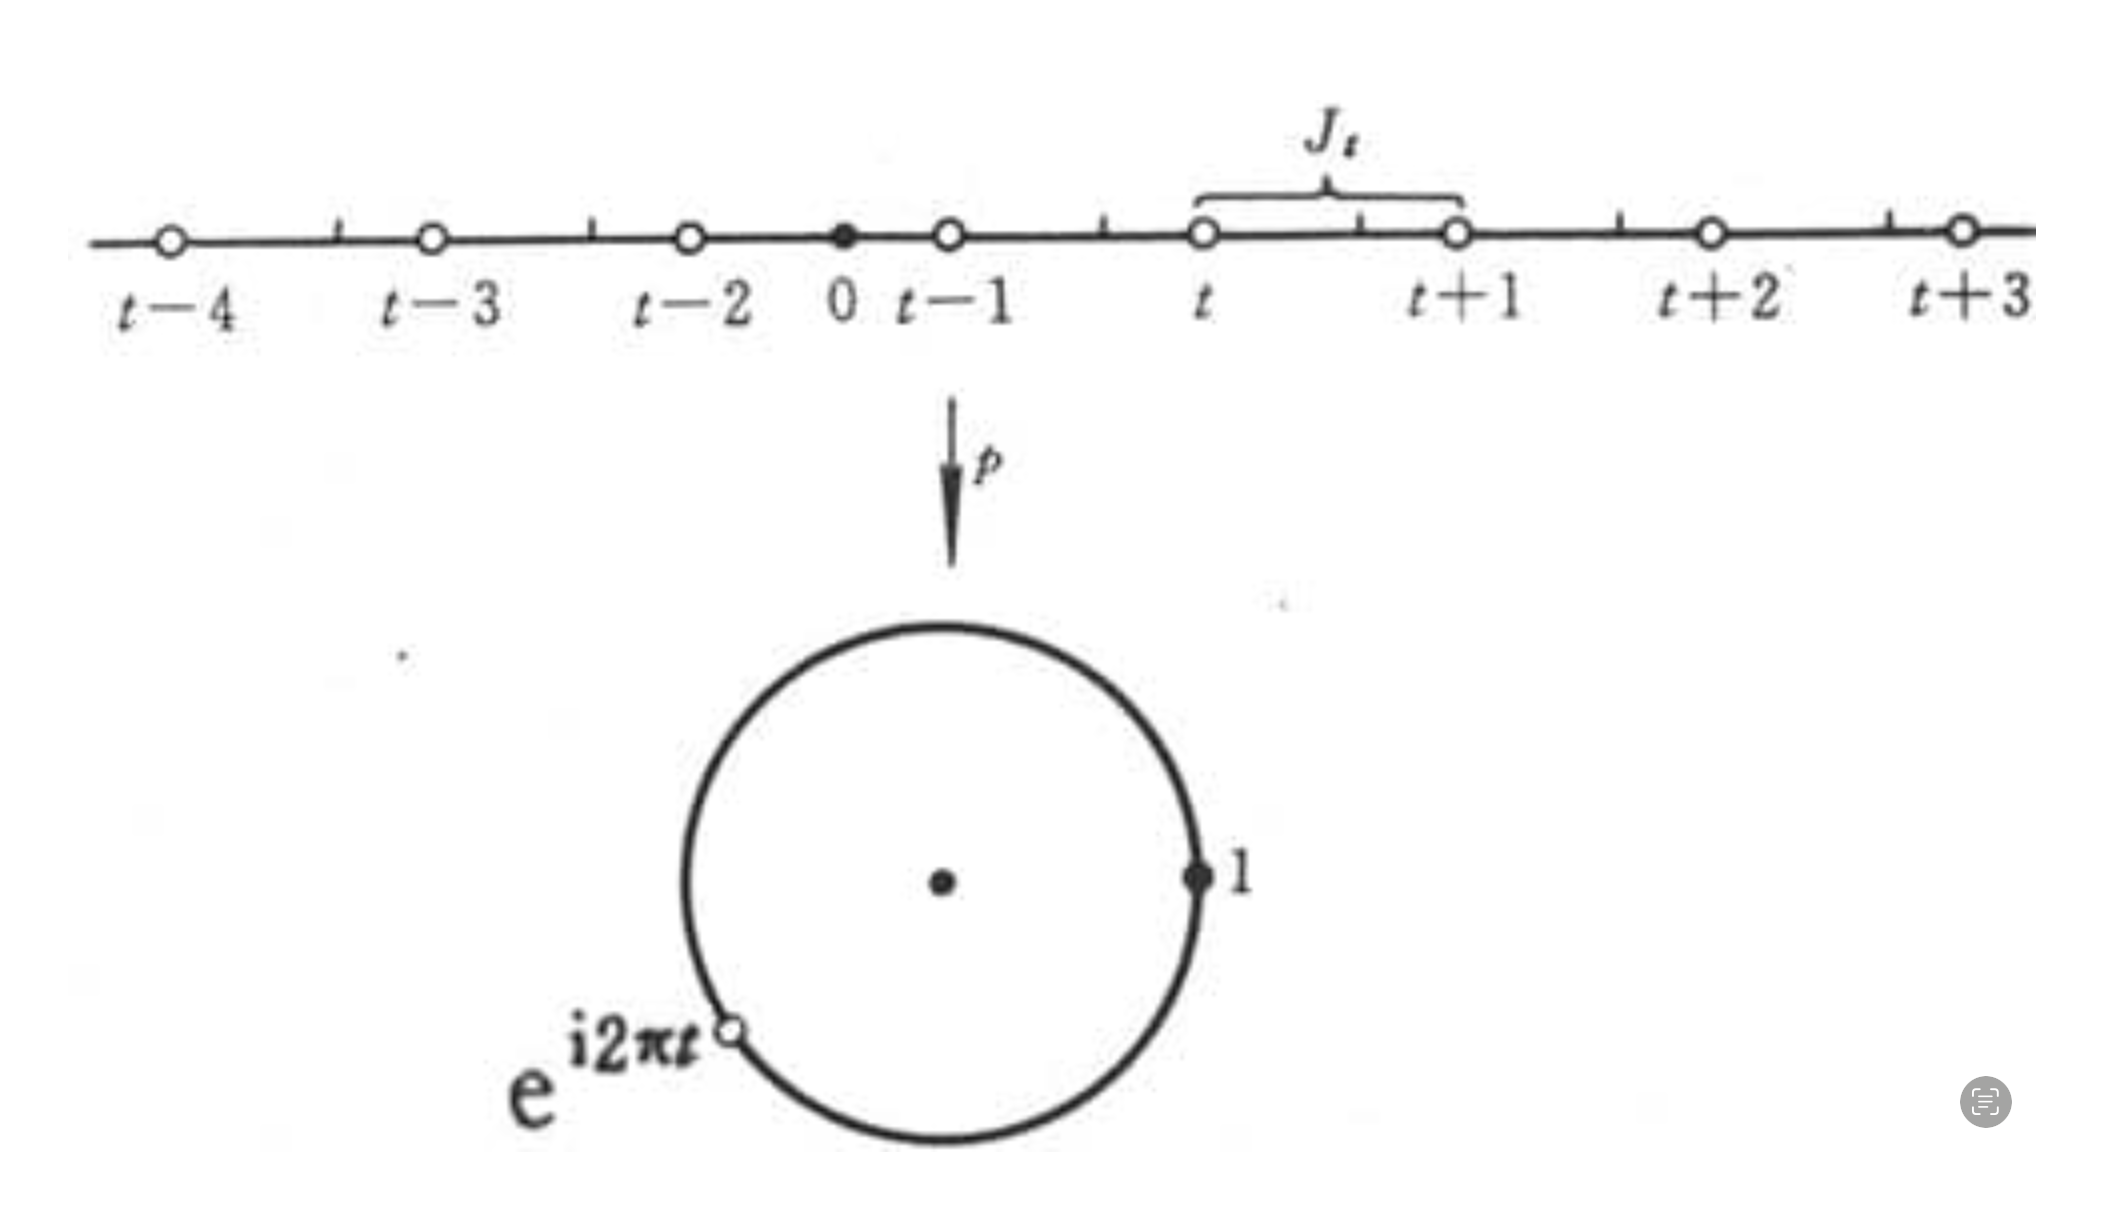
\includegraphics[width=0.5\linewidth]{image_23.png}
    \caption{}
    \label{fig:enter-label_23}
\end{figure}
\begin{lemma}
    如果f是非满映射,\(x_1 \in X , t_1 \in E^1\),使得\(p(t_1) = f(x_1)\),则存在f提升\(\widetilde{f}\),使得\[\widetilde{f}(x_1) = t_1\]
    如图\ref{fig:enter-label_24}
    \begin{figure}[H]
        \centering
        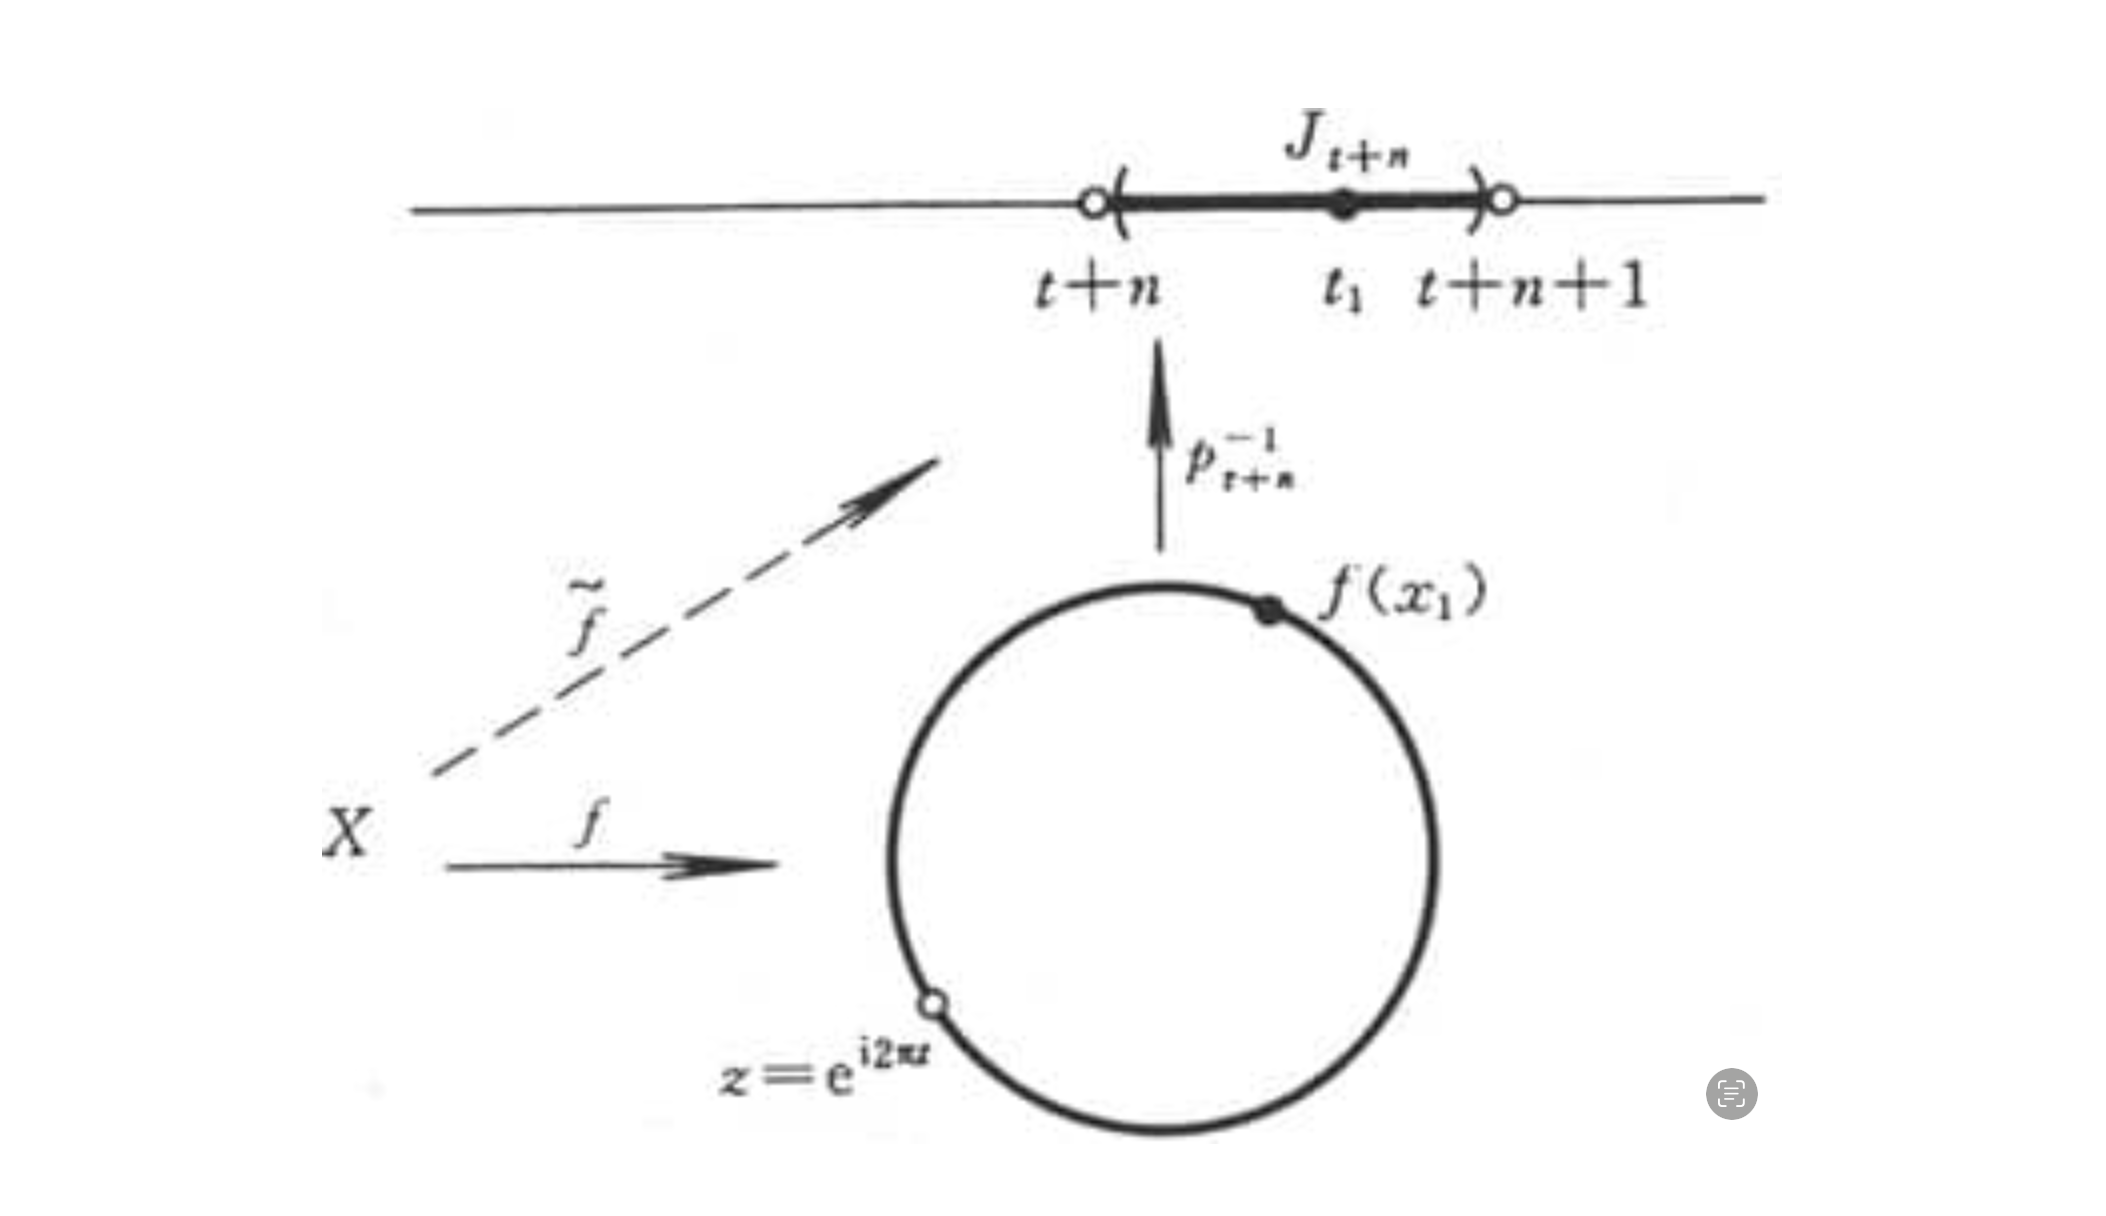
\includegraphics[width=0.5\linewidth]{image_24.png}
        \caption{}
        \label{fig:enter-label_24}
    \end{figure}
\end{lemma}
\begin{lemma}
    设a是\(S^1\)上的道路,\(t_0 \in E^1\)使得\(p(t_0) = a(0)\),则存在a的唯一提升\(\widetilde{a}\),使得\(\widetilde{a}(0) = t_0\).
\end{lemma}
\begin{lemma}
    设a,b是\(S^1\)上基点为\(z_0\)的两条闭路,使得\(\forall t \in I , a(t) \neq -b(t) \),则\(q(a) = q(b) \).
\end{lemma}
\begin{lemma}
    设a,b是\(S^1\)上基点为\(z_0\)的闭路,则\(q(a) =q(b) \Leftrightarrow a \underset{.}{\simeq} b \)
\end{lemma}
\begin{theorem}
    \(\pi_1(S^1 ,z_0)\)是自由循环群
\end{theorem}
\begin{proof}
    设\(a \in \pi_1 (S^1 ,z_0 )\) ,规定为\(q(a) =q(\alpha) \quad a \in \alpha\) ,使得映射\(q : \pi_1 (S^1 ,z_0) \rightarrow Z \)\\
    设\(\alpha = <a > \quad \beta = <b> \),作a,b的提升\(\widetilde{a}\)和\(\widetilde{b}\),使得\(\widetilde{a}(1) = \widetilde{b}(0)\)则\(\widetilde{a}\widetilde{b}\)是ab的提升,它的起,终点为\(\widetilde{a}(0) = \widetilde{b}(1)\),于是\begin{align*}
        q(\alpha\beta)&= \widetilde{b}(1)  - \widetilde{a}(0) \\
        &= \widetilde{b}(1) - \widetilde{b}(0) + \widetilde{a}(1) -\widetilde{a}(0) \\
        &= q(a) +q(b) = q(\alpha) + q(\beta)
    \end{align*}
    
\end{proof}
于是,我们可知\(\pi_1 (S^1 ,z_0)\)是由\(<\alpha_0 > \)生成的自由循环群.
\subsection*'{\(n \geq 2 \)时,\(S^n\)单连通}
\begin{corollary}
    设\(X_1 , X_2 \)都是X 的开集,其中\(X_2\)是单连通空间,并且\(X_1 \cup X_2 = X \quad X_1 \cap X_2\)非空且是道路连通空间,则有\(l_{\pi}: \pi_1(X_1 ,x_0) \rightarrow \pi_1v (X,x_0)\)是满同态,这里\(i: X_1 \rightarrow X \)是包含映射,\(x_0 \in X_1\).
\end{corollary}
\begin{proposition}
    若X是它的两个单连通开集\(X_1 , X_2\)的并集,并且\(X_1 \cap X_2\)非空,道路连通,则X也是单连通空间
\end{proposition}
\subsection*{\(T^2\)的基本群}
由于\(T^2 = S^1 \times S^1\)因此我们推测有如下定理: 
\begin{theorem}
    设\(x_0 \in X  \quad y_0 \in Y\),则
    \[\pi_1 (X \times Y , (x_0,y_0)) \cong \pi_1 (X,x_0) \times \pi_1 (Y, y_0)\]
\end{theorem}
\begin{proof}
    \begin{figure}[H]
        \centering
        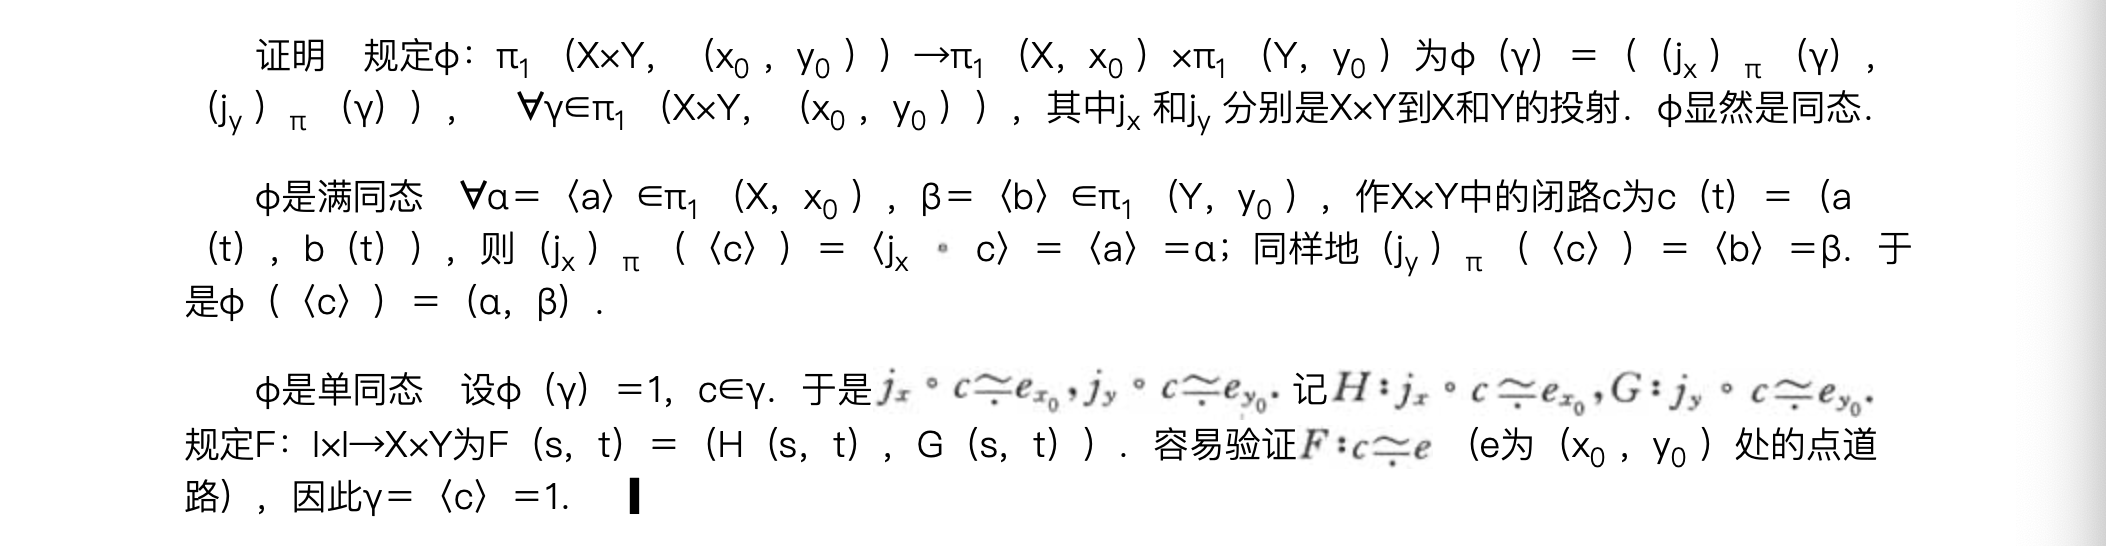
\includegraphics[width=0.5\linewidth]{image_25.png}
        \caption{定理证明}
        \label{fig:enter-label_27}
    \end{figure}
\end{proof}
上述定理应用到\(T^2\),可知: \(T^2 \cong Z \times Z \),从而对于任何正整数n 有:\(T^n \cong Z \times Z \times \dots \times Z = Z^n\)
并且有\(T^2 \not\cong S^2 \) 
\section{基本群的同伦不变性}
“本节穿插着讲两方面的内容:拓扑空间的同伦等价和基本群的同伦不变性.前者介绍拓扑空间集合中的一种新的等价关系,并讨论各种常用情况,它们都是代数拓扑学的重要的基本概念;后者包括同伦的映射导出的基本群同态间的关系以及基本群的伦型不变性,它们在基本群的计算和应用中起了十分重要的作用.”
\subsection*{同伦的映射导出的基本群同态间的关系}
设\(f \simeq g : X \rightarrow Y \),于是f可以逐渐地变为g,那么基本群同态\(f_{\pi}\)也可以逐渐地变为\(g_{\pi}\),也就是说\(f_{\pi}\)与\(g_{\pi}\)应该有着紧密的联系.
\\
取定\(x_0 \in X \),记\(y_0 =f(x_0), y_1 = g(x_0)\) .一般地来说\(y_0 \neq y_1 \),因此\(f_{\pi},g_{\pi}\)是从\(\pi_1 (X , x_0)\)分别到不同群\(\pi_1 (Y, y_0)\)到\(\pi_1 (Y,y_1)\)的两个同态.设\(H: f \simeq  g\) , 由\(w(t) = H(x_0 ,t) , \quad t \in I \),规定Y中从\(y_0\)到\(y_1\)的道路w,称为H在\(x_0\)处的踪,记\(w =<w>\),因此有同构\(w_{\#}: \pi_1 (Y,y_0) \rightarrow \pi_1 (Y,y_1)\)
\begin{theorem}
    \(g_{\pi}=w_{\#} * f_{\pi} : \pi_1 (X,x_0) \rightarrow \pi_1 (Y,y_1)\),即图表可交换(图\ref{fig:enter-label_26}).
    \begin{figure}[H]
        \centering
        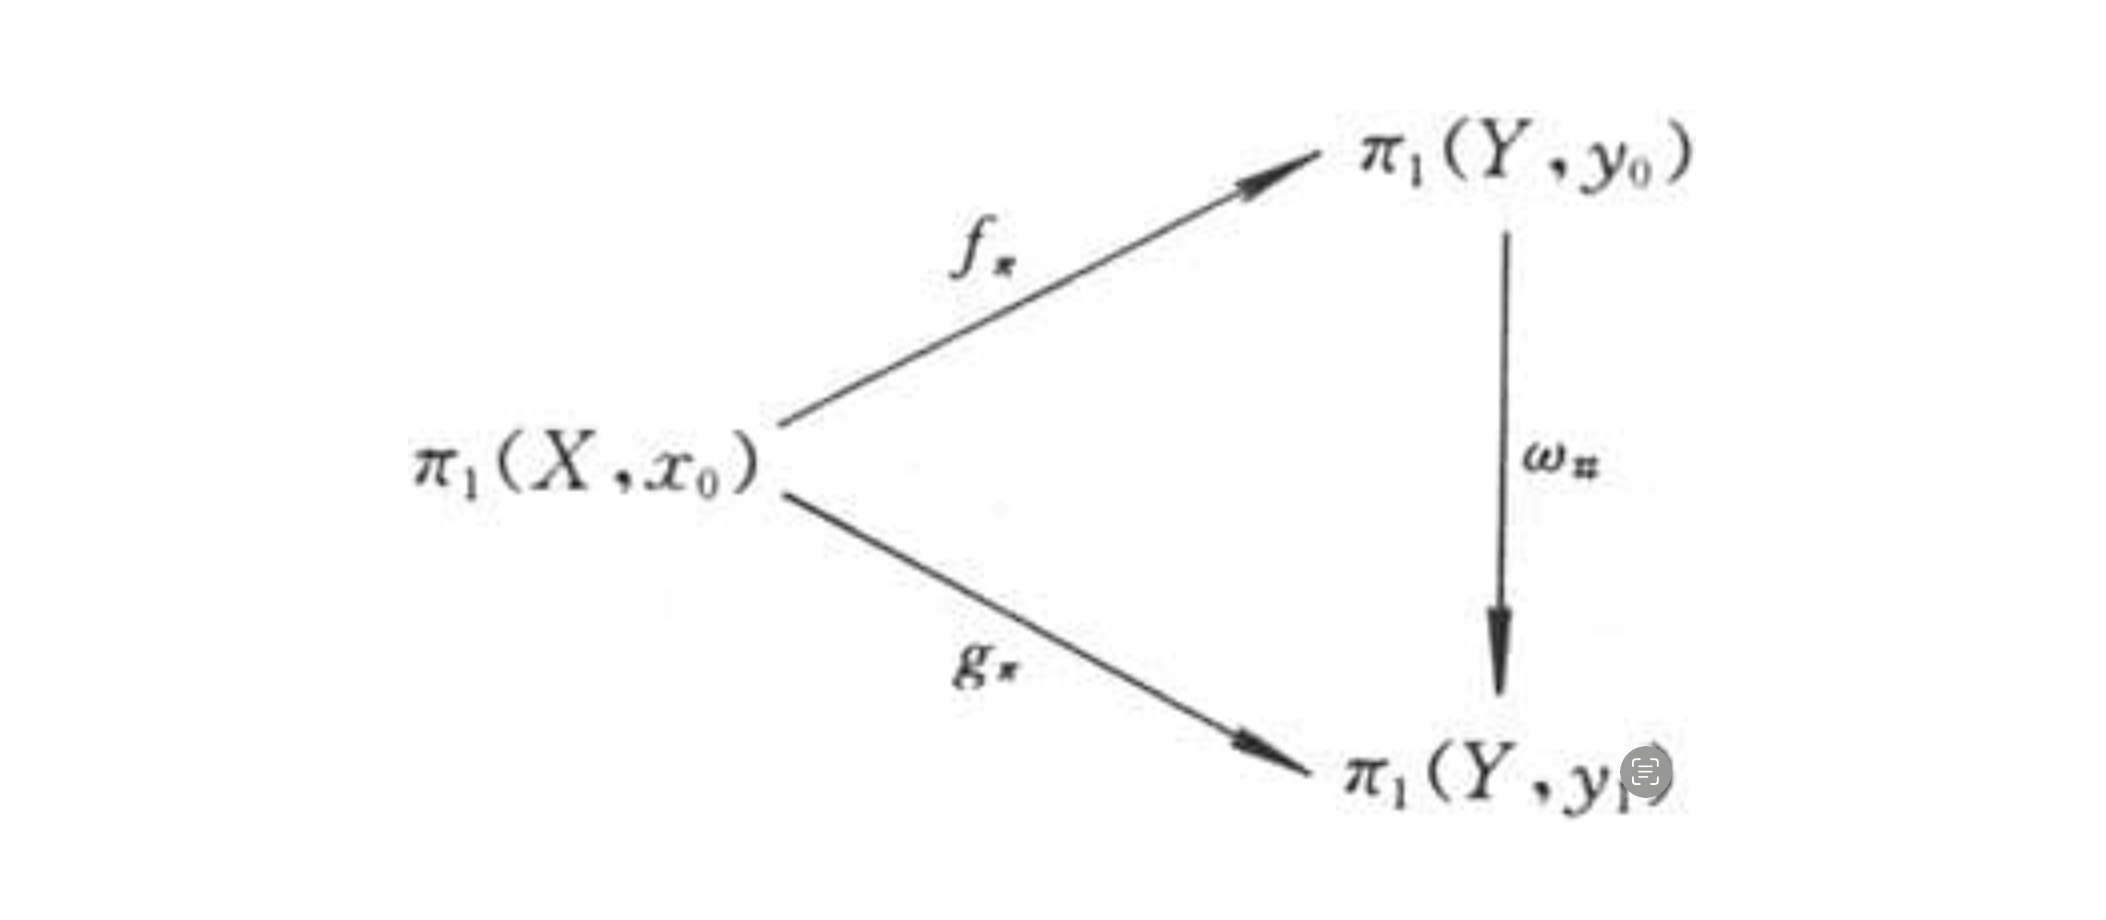
\includegraphics[width=0.5\linewidth]{image_26.png}
        \caption{}
        \label{fig:enter-label_26}
    \end{figure}
\end{theorem}
上述定理说明:当\(f \simeq g \)时,\(f_{\pi}\)与\(g_{\pi}\)相差一个同构,因此它们会具有许多共同的性质.
\subsection*{拓扑空间的同伦等价}
\begin{definition}
    设X与Y为两个拓扑空间,如果存在连续映射\(f: X \rightarrow Y \)和\(g: Y \rightarrow X \),使得\begin{align*}
        g*f &\simeq id_{X} : X \rightarrow X  \\
        f*g &\simeq id_{Y} : Y \rightarrow Y 
    \end{align*}
    则说X与Y是同伦等价的(或者称它们具有相同的伦型),记作\(X \simeq Y \),称f和g为同伦等价(映射),称g是f的一个同伦逆,反之f也是g的同伦逆.
\end{definition}
\begin{note}
    同胚映射的逆是唯一的,而同伦等价(映射)的同伦逆却不是唯一的,它们构成一个映射类.
\end{note}
\begin{corollary}
    若\(f: X \rightarrow Y \)是同伦等价,\(x_0 \in X \quad y_0 =f(x_0)\),则\(f_{\pi} : \pi_1 (X,x_0) \rightarrow \pi_2 (Y,y_0)\)是同构.
\end{corollary}
\begin{proposition}
    若\(X \simeq Y \)且它们都是道路连通空间,则\(\pi_1(X) \cong \pi_1 (Y)\)
\end{proposition}
给出利用这个推论的两个例子
\begin{example}
    求平环的基本群,并判断它和\(D^2\)是否是同伦等价.
\end{example}
\begin{solution}
    由于平环同胚于\(S^1\)同时\(\pi_1 (S^1) \cong Z \),从而得到平环的基本群也是自由循环群,那么可知平环与\(D^2\)不同伦等价\end{solution}
\subsection*{形变收缩核}
\begin{definition}
    设A是X的子空间,\(I : A \rightarrow X \)是包含映射,如果存在收缩映射\(r : X \rightarrow A \)(即\(r* i = id_A : A \rightarrow A \),使得\(i * r \simeq id_X : X \rightarrow X  \),就称A是X的一个形变收缩核.
\end{definition}
下面给出形变收缩核的映射连续变化:
\begin{definition}
    对于连续映射H来说,A是X的子空间且\(H: X \times I \rightarrow X \)如果满足: 
    \begin{enumerate}
        \item \(H(x,0) = x  \quad \forall x \in X \) \\
        \item \(H(x,1) \in A  \quad \forall x \in  X\) \\
        \item \(H(a,1) = a  \quad \forall a \in A \)
    \end{enumerate}
    则称H是X到A的一个形变收缩
    \end{definition}
    于是,当A是X的形变收缩核时,就存在从X到A的形变收缩.反之,当H是从X到A的形变收缩时,可规定收缩映射\(r: X \rightarrow A\),使得\(i*r(x)= H(x,1) \),则\(H: id_X \simeq i * r\),从而A时X的形变收缩核.因此,形变收缩核与形变收缩只是同一件事的两种不同定义方式,它们分别从空间和映射着两个不同角度作描述.
    \begin{example}
        把乘积空间\(X \times I \)的子集\(X_s = X \times \left\{s\right\}\)称为它的s-切片都是\(X \times I \)的形变收缩核
    \end{example}
    \begin{solution}
        确定\(s_0\),则\(X \times I\)到\(X_{s_0}\)的一个形变收缩可规定为\[H(x,s,t) = (X , (1-t)s+ts_0)\]
    \end{solution}
    \begin{example}
        \(S^{n-1}\)是\(E^{n} \setminus \left\{o\right\}\)的形变收缩核,则形变收缩H可规定为\[H(x,t) = (1-t)x + t\frac{x}{||x||}\]
        相应的收缩映射是由\(r(x) = \frac{x}{||x||}\)所规定的映射(如图\ref{fig:enter-label_27})
        \begin{figure}[H]
            \centering
            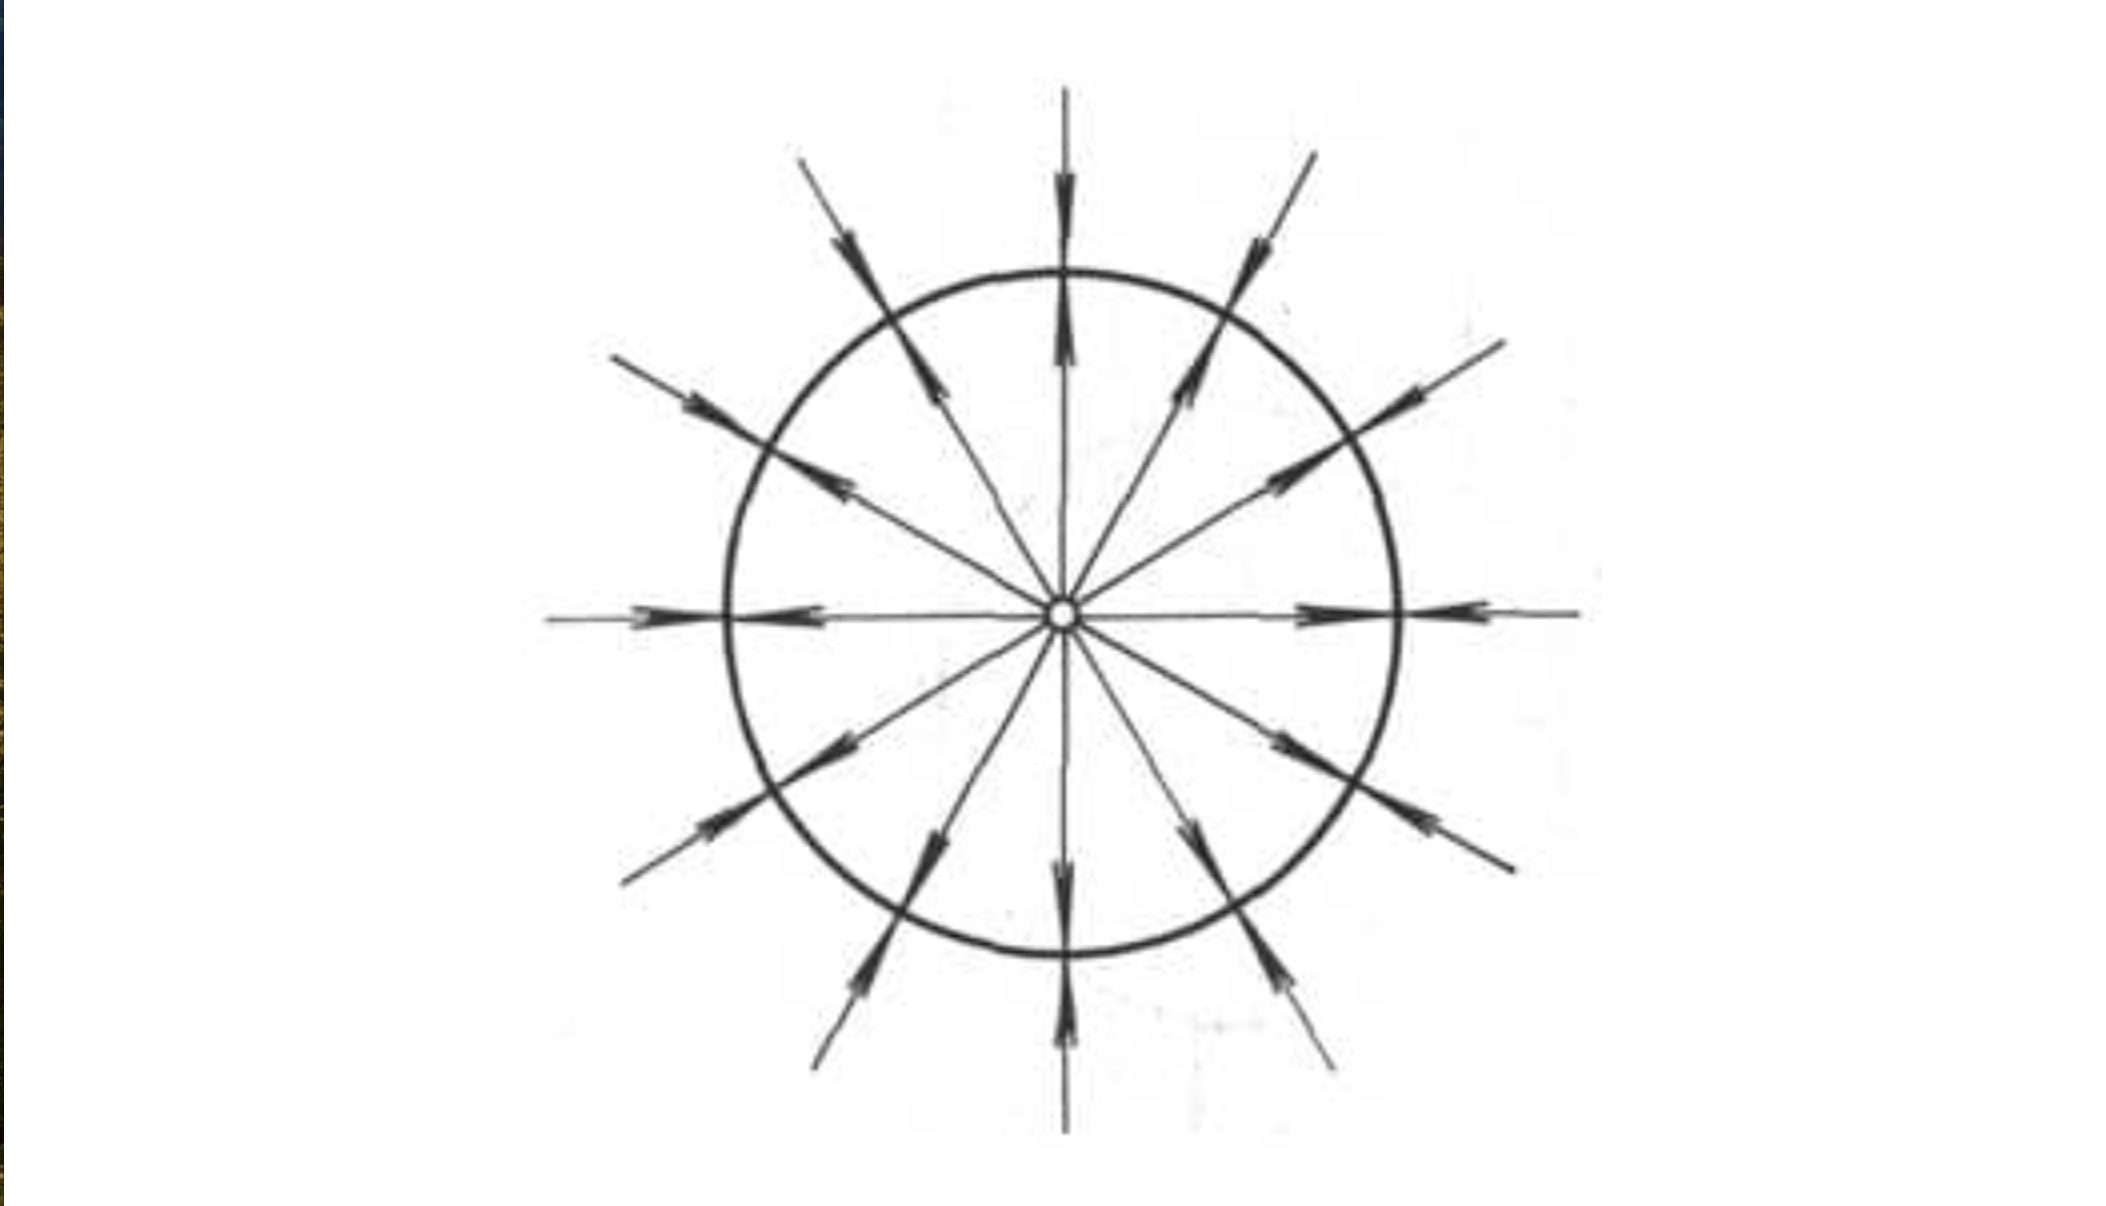
\includegraphics[width=0.5\linewidth]{image_27.png}
            \caption{}
            \label{fig:enter-label_27}
        \end{figure}
        如果\(X \subset E^n\),A是X的子集,且有收缩映射\(r: X \rightarrow A \).使得\(\overline{xr(x)} \subset X \quad \forall x \in X \) ,则\(i*r\)与\(id_X\)间可建立直线同伦,因而A是X的形变收缩核,特别地,当X时凸集时,它的每个收缩核都是形变收缩核.
    \end{example}
    \begin{definition}
        X到A的一个形变收缩H如果保持A中的点不动,即形变收缩定义中的条件(3)改成\[H(a,t) =a \quad \forall a \in A , t \in I \]
        则称H是一个强形变收缩,称A是X的强形变收缩核.这时有\(H : id_X \simeq i *r \quad relA \),于是,强形变收缩就是保持形变收缩核中的每一个点不动的形变收缩.
    \end{definition}
    \begin{corollary}
        设\(f: X \rightarrow Y\)是商映射,\(A \subset X \quad B=f(A)\),如果H是X到A的(强)形变收缩,并且满足条件:当\(x \overset{f}{\sim} x^{'}\)时,\(\forall t \in I \),\(H(x,t) \overset{f}{\sim}H(x^{'}, t)\)则存在Y到B的(强)形变收缩.
    \end{corollary}
    \begin{theorem}
        任何闭曲面去掉一点后,可强形变收缩为曲面上的一个圆束(即两两相交于同一点的一组圆周的并集)\(\bigcup_{i=1}^n S^1_i\)其中\[k=\begin{cases}
            2n \quad &\text{若闭曲面是} nT^2 \text{型} \\
            m  \quad &\text{若闭曲面是} mp^2 \text{型}
        \end{cases}\]
    \end{theorem}
\subsection*{可缩空间}
可缩空间是伦型最简单的一类空间.
\begin{definition}
    与单点空间同伦等价的拓扑空间称为可缩空间.
\end{definition}
所有可缩空间构成一个空间的同伦等价类,它是最简单的一个等价类,可缩空间是道路连通的并且是单连通空间
\begin{corollary}
    如果X是可缩空间,则\(\forall x \in X \)都是X的形变收缩核
\end{corollary}
\subsection*{基本群的计算与应用}
\begin{theorem}[Van-Kampen定理]
如果拓扑空间X可分解为两个开集\(X_1\)与\(X_2\)之并,并且\(X_0 = X_1 \cap X_2\)非空且道路连通,则\(\forall X_0 \in X_0\),有
\[\pi_1 (X, x_0) \cong \pi_1(X_1 ,x_0) * \pi_1 (X_2 ,x_0) \setminus [\left\{(i_1)_{\pi}(a) (i_2)_{\pi}(a^{-1}) | a \in \pi_1 (X_0,x_0) \right\}]\]
其中\(i_i : X_0 \rightarrow X_i (i=1.2)\)是包含映射
\end{theorem}
\begin{theorem}
    如果上述定理中\(X_1 ,X_2\)都改为闭集,并且\(X_0\)是它的一个开邻域的强形变收缩核,其他条件不变则结论仍然成立.
\end{theorem}